\documentclass[tikz,border=4pt]{standalone}
\usepackage{amsmath,amssymb,bm}
\usepackage[T1]{fontenc}
\usepackage{newtxtext,newtxmath}
\usepackage{microtype}
\usepackage{tikz}
\usetikzlibrary{arrows.meta,positioning,calc,fit,backgrounds}

\definecolor{headLine}{HTML}{172033}
\definecolor{ink}     {HTML}{172033}
\definecolor{mutedInk}{HTML}{6B7280}
\definecolor{greyLine}{HTML}{9CA3AF}
\definecolor{greyFill}{HTML}{EEF0F3}
\definecolor{qkC}     {HTML}{B91C1C}
\definecolor{qkFill}  {HTML}{FEE2E2}
\definecolor{ovC}     {HTML}{0B7285}
\definecolor{ovFill}  {HTML}{E3F3F6}
\definecolor{saeC}    {HTML}{46378A}
\definecolor{saeFill} {HTML}{EEEAF8}
\definecolor{lambdaC} {HTML}{D9468F}
\definecolor{lambdaFill}{HTML}{FCE7F3}

\tikzset{
  >=Latex,
  every node/.append style={line join=round},
  attnBox/.style={draw=none,fill=none,inner sep=6mm},
  nodeOV/.style={draw=ovC,line width=0.85pt,rounded corners=2.2pt,
                 fill=ovFill,font=\normalsize\bfseries,text=ovC,
                 inner sep=3pt,minimum height=6mm,minimum width=14mm,align=center},
  nodeGrey/.style={draw=greyLine,line width=0.85pt,rounded corners=2.2pt,
                   fill=greyFill,font=\normalsize\bfseries,text=mutedInk,
                   inner sep=3pt,minimum height=6mm,minimum width=14mm,align=center},
  ovflow/.style={-{Latex[length=3.0mm,width=2.2mm]},line width=0.95pt,ovC,line cap=round},
  ovline/.style={line width=0.95pt,ovC,line cap=round},
  greyflow/.style={->,line width=0.9pt,greyLine,line cap=round},
  greyline/.style={line width=0.9pt,greyLine,line cap=round},
  saeBox/.style={draw=saeC,line width=0.95pt,rounded corners=4pt,
                 fill=saeFill,inner sep=3mm},
  feat/.style={draw=saeC!62,line width=0.45pt,fill=white,
               minimum width=5mm,minimum height=5mm,inner sep=0pt,
               font=\scriptsize\bfseries},
  featLambda/.style={draw=lambdaC,line width=1.15pt,fill=lambdaFill,
                 minimum width=5mm,minimum height=5mm,inner sep=0pt,
                 font=\small\bfseries,text=lambdaC},
  lambdaFlow/.style={-{Latex[length=3.0mm,width=2.2mm]},line width=0.95pt,lambdaC,line cap=round},
  lambdaTrace/.style={line width=0.9pt,lambdaC,line cap=round,line join=round},
}

\begin{document}
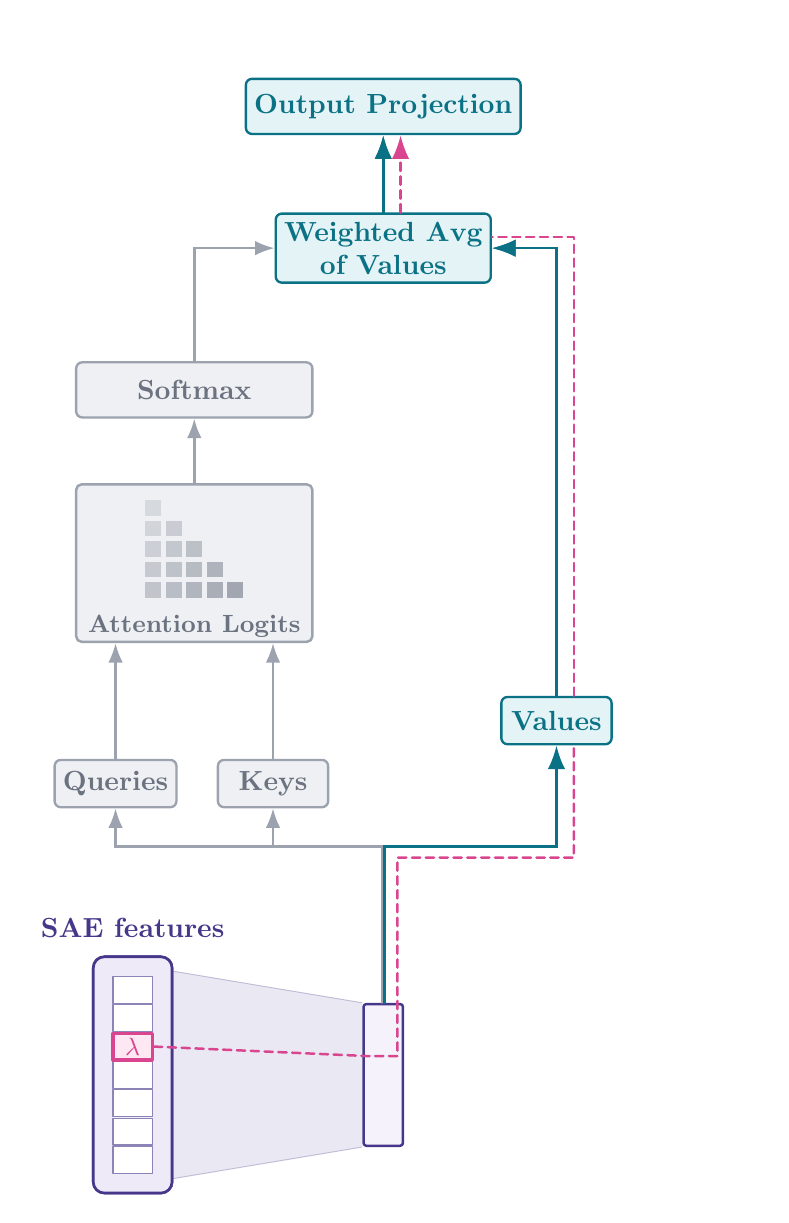
\begin{tikzpicture}[x=1mm,y=1mm]

% Same attention-head layout as the QK interaction diagram, with QK greyed out.
\node[nodeGrey] (queries) at (-22,34) {Queries};
\node[nodeGrey] (keys)    at (-2,34)  {Keys};
\node[nodeOV]   (values)  at (34,42)  {Values};

\node[draw=greyLine,line width=0.9pt,rounded corners=2pt,fill=greyFill,
      minimum width=30mm,minimum height=20mm,inner sep=1mm]
      (logits) at (-12,62) {};
\node[font=\small\bfseries,mutedInk,anchor=south,inner sep=1pt]
  at ([yshift=0.3mm]logits.south) {Attention Logits};

\pgfmathsetmacro{\HC}{2.6}
\foreach \r in {0,...,4} {%
  \foreach \c in {0,...,4} {%
    \pgfmathtruncatemacro{\active}{\c <= \r ? 1 : 0}%
    \pgfmathsetmacro{\op}{\active * (0.18 + 0.10*\c + 0.04*(\r-\c))}%
    \pgfmathsetmacro{\xc}{(\c-2)*\HC}%
    \pgfmathsetmacro{\yc}{1.8 + (2-\r)*\HC}%
    \fill[mutedInk,opacity=\op]
      ([xshift=\xc mm-1mm,yshift=\yc mm-1mm]logits.center)
      rectangle
      ([xshift=\xc mm+1mm,yshift=\yc mm+1mm]logits.center);
  }%
}

\node[nodeGrey,minimum width=30mm,minimum height=7mm]
      (softmax) at (-12,84) {Softmax};
\node[nodeOV] (wavg) at (12,102) {Weighted Avg\\ of Values};
\node[nodeOV,minimum width=30mm,minimum height=7mm]
      (oproj) at (12,120) {Output Projection};

\coordinate (jx) at (12,26);
\coordinate (jxQK) at ([xshift=-0.18mm]jx);
\coordinate (jxOV) at ([xshift=0.18mm]jx);
\draw[greyflow] (jxQK) -| (keys.south);
\draw[greyflow] (jxQK) -| (queries.south);
\draw[ovflow] (jxOV) -| (values.south);

\draw[greyflow] (keys.north)    -- (keys.north    |- logits.south);
\draw[greyflow] (queries.north) -- (queries.north |- logits.south);
\draw[greyflow] (logits.north) -- (softmax.south);
\draw[greyflow] (softmax.north) -- ++(0,3) |- (wavg.west);
\draw[ovflow] (values.north) |- (wavg.east);
\draw[ovflow,line width=1.1pt] (wavg.north) -- (oproj.south);

\coordinate (xTop) at (12,16);
\coordinate (outTop) at (54,124);
\begin{scope}[on background layer]
  \node[attnBox,fit=(keys)(values)(logits)(softmax)(wavg)(oproj)(xTop)(outTop)] (head) {};
\end{scope}

% SAE expanded into the activation block, with only lambda highlighted.
\node[draw=saeC,line width=0.9pt,rounded corners=1pt,fill=saeFill!60,
      minimum width=5mm,minimum height=18mm,inner sep=0pt]
      (postLNvec) at (12,-3) {};

\draw[greyline]
  ([xshift=-0.18mm]postLNvec.north) -- (jxQK) -- (keys.south |- jx);
\draw[ovline]
  ([xshift=0.18mm]postLNvec.north) -- (jxOV) -- (values.south |- jx);

\node[saeBox,minimum width=10mm,minimum height=30mm,
      left=24mm of postLNvec.west,anchor=east] (sae) {};

\begin{scope}[on background layer]
  \fill[saeC!38,opacity=0.30]
    (postLNvec.north west) -- ([yshift=-2mm]sae.north east) --
    ([yshift=2mm]sae.south east) -- (postLNvec.south west) -- cycle;
  \draw[saeC!55,opacity=0.55,line width=0.35pt]
    (postLNvec.north west) -- ([yshift=-2mm]sae.north east);
  \draw[saeC!55,opacity=0.55,line width=0.35pt]
    (postLNvec.south west) -- ([yshift=2mm]sae.south east);
\end{scope}

\node[saeBox,minimum width=10mm,minimum height=30mm,
      left=24mm of postLNvec.west,anchor=east] (sae) {};

\foreach \i in {1,...,7} {
  \node[feat,minimum width=5mm,minimum height=3.4mm]
        (f\i) at ([yshift={(\i-4)*3.6mm}]sae.center) {};
}
\node[featLambda,minimum height=3.4mm] (flam) at (f5.center) {$\lambda$};

\node[font=\normalsize\bfseries,saeC,align=center,above=1mm of sae.north,anchor=south]
  {SAE features};

% Lambda follows the OV channel through values into the weighted average.
\coordinate (lamStem) at ([xshift=1.8mm]postLNvec.north);
\coordinate (lamEntry) at ([xshift=0.5mm,yshift=2.4mm]postLNvec.west);
\coordinate (lamInside) at (lamStem |- lamEntry);
\coordinate (lambdaOVBase) at ([xshift=1.8mm]postLNvec.north);
\coordinate (lambdaValueBase) at ([xshift=2.2mm]values.south);
\coordinate (lambdaValueTop) at ([xshift=2.2mm]values.north);
\coordinate (lambdaWavgSide) at ([yshift=1.4mm]wavg.east);
\coordinate (lambdaWavgTop) at ([xshift=2.2mm]wavg.north);
\coordinate (lambdaOprojTarget) at ([xshift=2.2mm]oproj.south);

\draw[lambdaTrace,densely dashed]
  (flam.east) -- (lamEntry) -- (lamInside) -- (lamStem) -- (lambdaOVBase)
  -- ([yshift=-1.4mm]lambdaOVBase |- jx)
  -- ([xshift=2.2mm,yshift=-1.4mm]values.south |- jx)
  -- (lambdaValueBase);
\draw[lambdaTrace,densely dashed]
  (lambdaValueTop) -- (lambdaValueTop |- lambdaWavgSide) -- (lambdaWavgSide);
\draw[lambdaFlow,densely dashed]
  (lambdaWavgTop) -- (lambdaOprojTarget);
\draw[ovflow] (values.north) |- (wavg.east);
\draw[ovflow,line width=1.1pt] (wavg.north) -- (oproj.south);

\end{tikzpicture}
\end{document}
